\documentclass[11pt]{beamer}
\usetheme{PaloAlto}
\usecolortheme{spruce}
\usepackage[spanish]{babel}
\usefonttheme{professionalfonts}
\usefonttheme{serif}
\usepackage{minted}
\usepackage{fontspec}
\setmainfont{Liberation Serif}
\usepackage{amsmath}
\usepackage{amsfonts}
\usepackage{amssymb}
\usepackage{graphicx}
%Se configura minted
\definecolor{bg}{rgb}{0.95,0.95,0.95}
%\newminted{python}{fontsize=\scriptsize, 
%		   linenos,
%		   numbersep=8pt,
%		   gobble=4,
%		   frame=lines,
%		   bgcolor=bg,
%		   framesep=3mm} 
%\newminted{pycon}{bgcolor=bg, linenos=true, tabsize=4}
\newcommand{\tab}[1][1cm]{\hspace*{#1}}

\author{Nelson David Pérez Garecía\\}
\title{Introducción a Python y Obspy:\\Sesión I}
%\setbeamercovered{transparent} 
%\setbeamertemplate{navigation symbols}{} 
%\logo{} 
\institute{Servicio Geológico Colombiano} 
\date{} 
%\subject{} 
\begin{document}

\begin{frame}
\titlepage
\begin{center}
\begin{figure}

\includegraphics[scale=0.15]{Logo-SGC.jpg}
\end{figure}
\end{center}
\end{frame}

\begin{frame}
\tableofcontents
\end{frame}

\section{Introducción}
\subsection{Antes de comenzar}
\begin{frame}{Antes de comenzar...}
Algunos conceptos básicos:
\begin{itemize}
\item Para comunicarnos usamos sistemas estructurados bajo ciertas reglas en un contexto determinado. Estos sistemas son conocidos como lenguajes.
\pause
\item Existen lenguajes naturales y lenguajes formales. 
\pause
\item \textbf{Los lenguajes de programación son lenguajes formales que se diseñaron para expresar cálculos.}
\pause
\item Un programa es una secuencia de instrucciones que especifica cómo realizar un cálculo. Poseen instrucciones básicas cómo \textit{entrada, salida, operaciones matemáticas, ejecuciones condicionales, repeticiones.}
\pause
\item Un script es un archivo que contienen las instrucciones (código) qué pueden ser ejecutas por un itérprete.
\end{itemize}
\end{frame}

\begin{frame}{Antes de comenzar...}
Existen distintos tipos y clasificaciones para lenguajes de programación:
\begin{itemize}
\item Lenguajes de bajo nivel (``assembler``) y lenguajes de alto nivel (C++, C, Java, Perl, Bash, \textbf{Python}).
\pause
\item Lenguajes con diferente {\it paradigma} de programación: orientados a objetos, imperativos, funcionales.
\pause
\item Lenguajes compilados (C, C++, Fortran) y lenguajes interpretados (Bash, \textbf{Python}).
\end{itemize}
\end{frame}

\begin{frame}
\begin{figure}
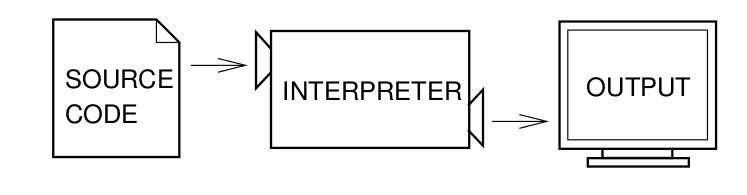
\includegraphics[scale=0.3]{interpretado.png}
\caption{Esquema de lenguaje interpretado}
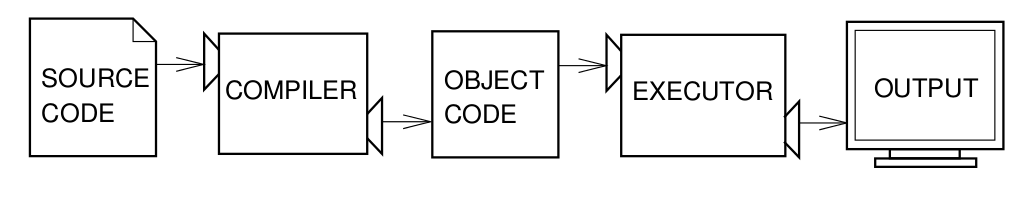
\includegraphics[scale=0.3]{compilado.png}
\caption{Esquema de lenguaje compilado}
\end{figure}
\end{frame}

\subsection{¿Qué es Python?}
\begin{frame}
\begin{center}
\begin{huge}
¿QUÉ ES PYTHON?
\end{huge}
\end{center}
\end{frame}

\begin{frame}{¿Qué es python?}
Python es un lenguaje de programación diseñado por Guido Van Rossum. Su primera versión se publicó en 1991 y actualmente cuenta con dos versiones estables 2.7 y 3.5
\begin{figure}
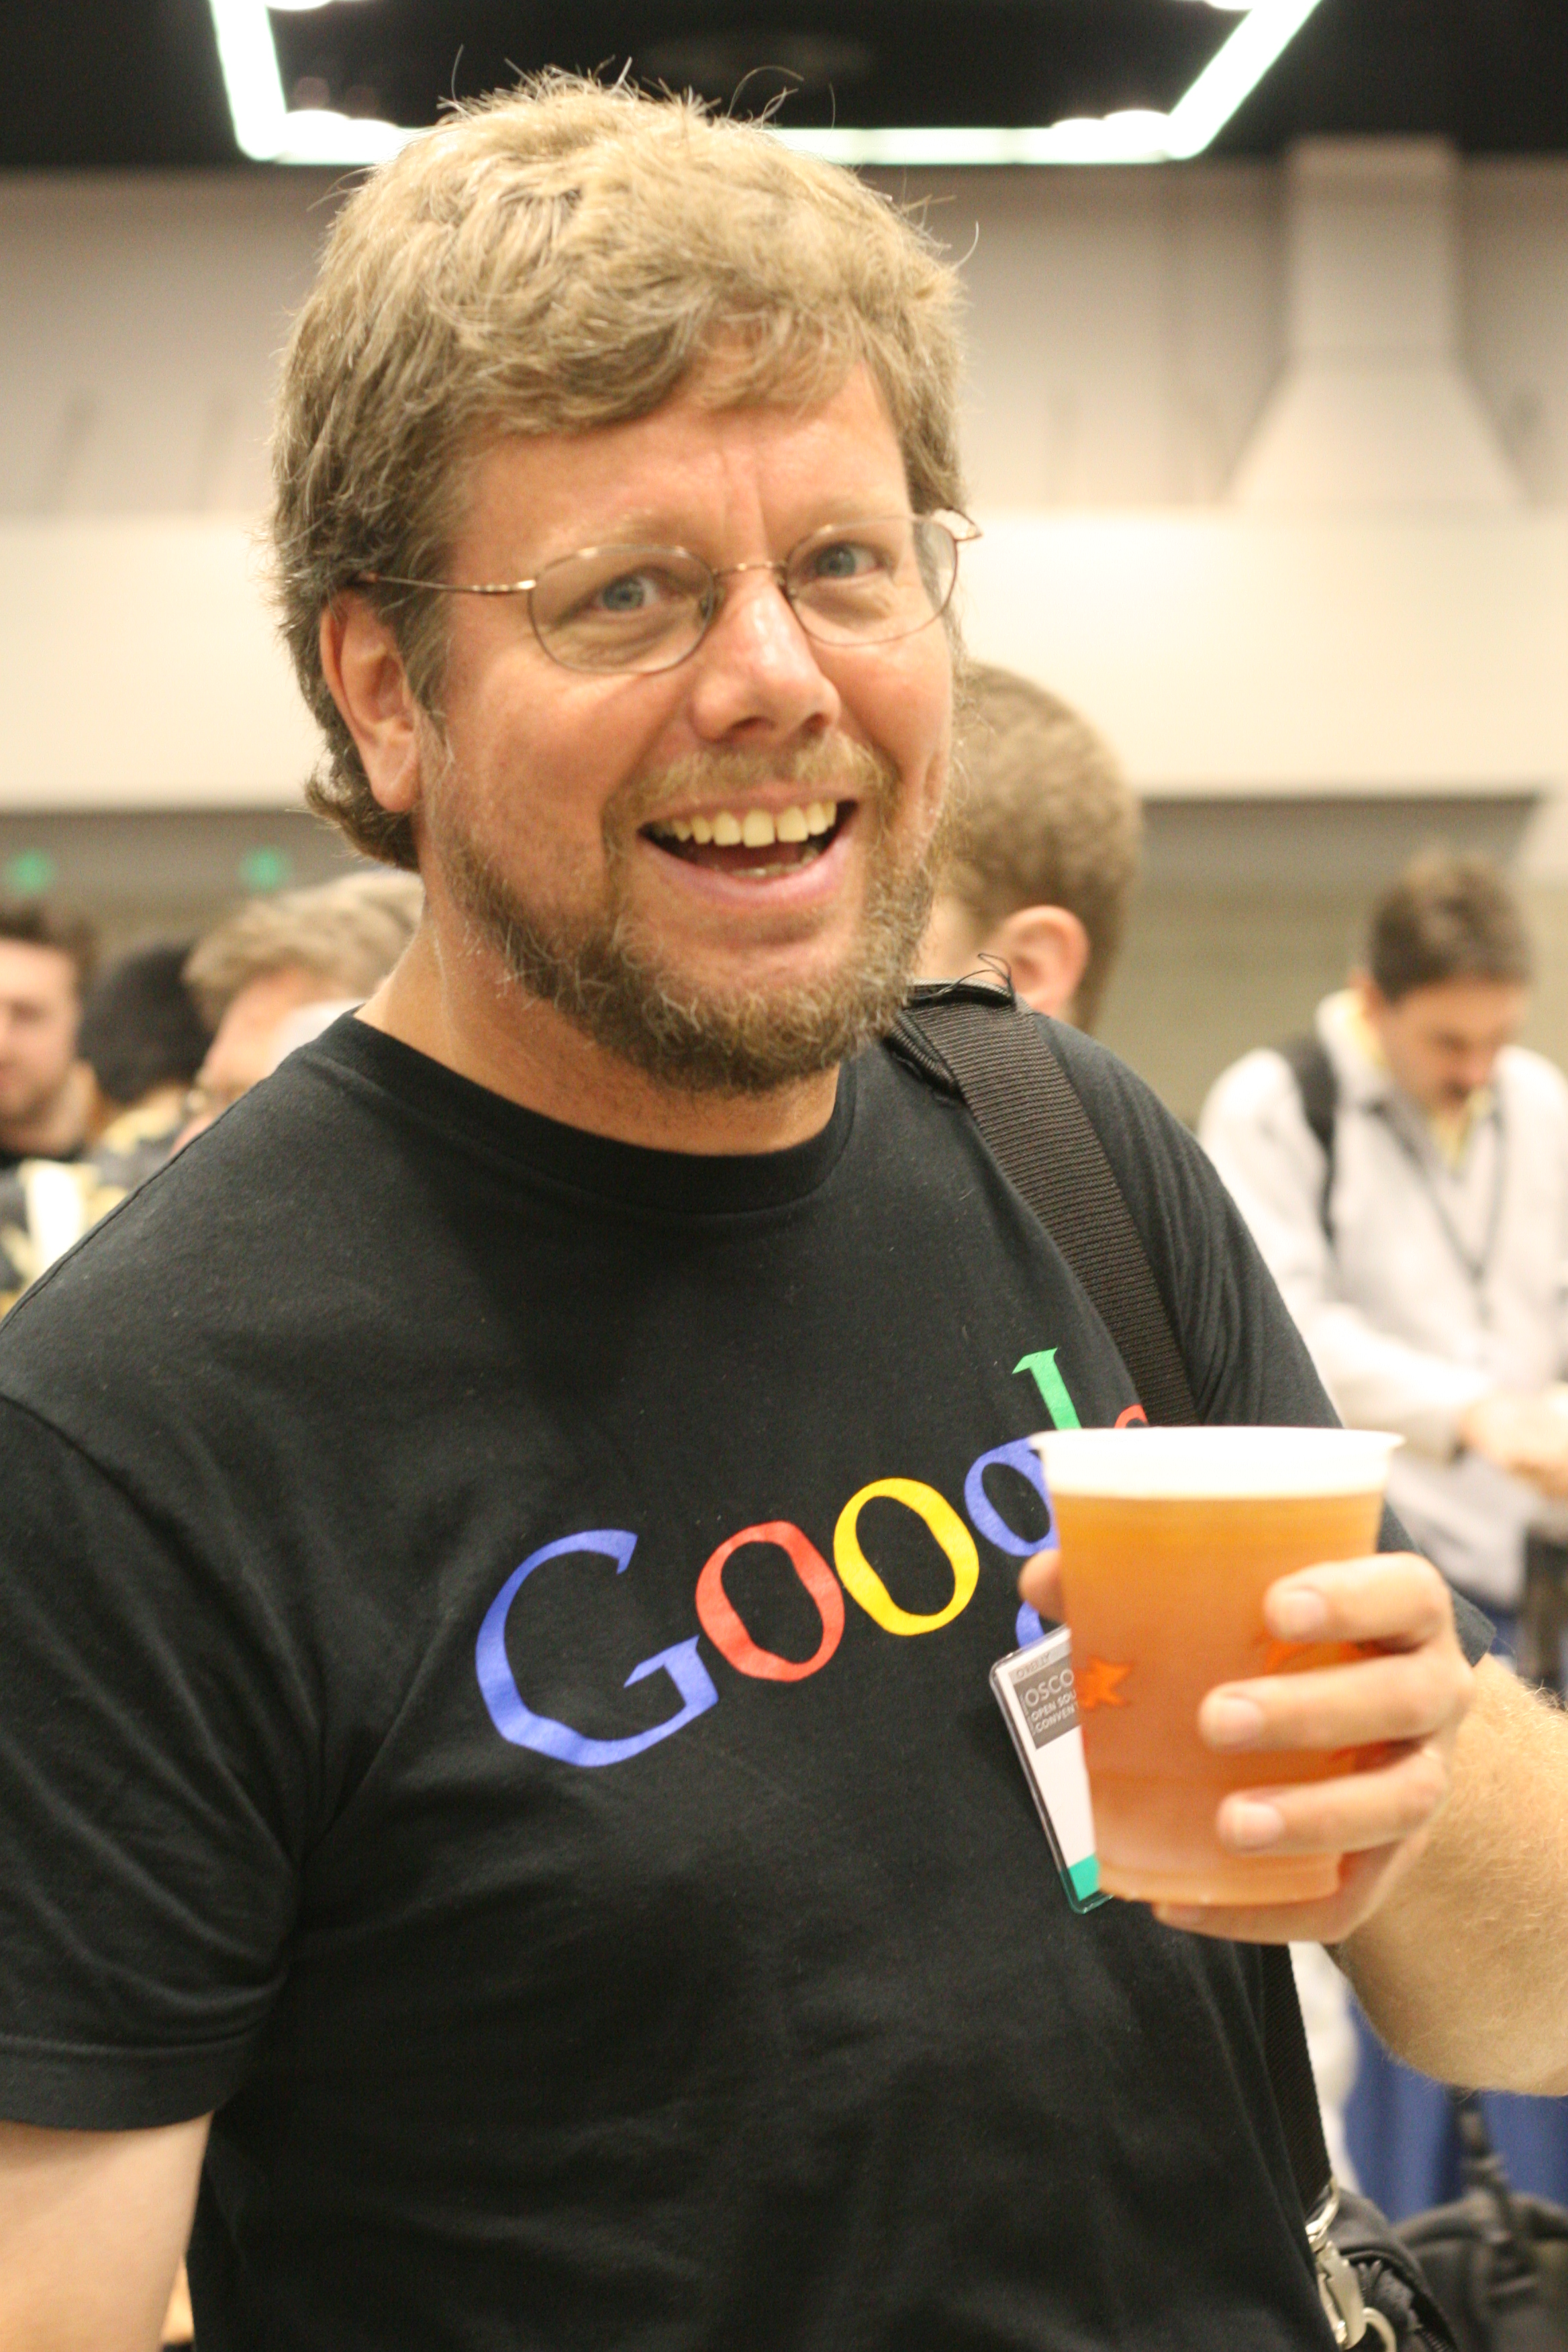
\includegraphics[scale=0.03]{guido.jpg}
\caption{Benevolente Dictador Vitalicio}

\includegraphics[scale=0.2]{python-logo.png}
\end{figure}
\end{frame}

\begin{frame}{Características}
\begin{itemize}
\item \textbf{Python} es un lenguaje de programación de alto nivel interpretado.
\pause
\item \textbf{Python} es portable. Los programas se pueden ejecutar en distintas plataformas sin (muchas) modificaciones.
\pause
\item \textbf{Python} es multiparadigma. Permite programación orientada a objetos y programación imperativa.
\pause
\item Posee licencia de código abierto compatible con la licencia general de GNU.
\end{itemize}
\end{frame}

\begin{frame}{Instalación}
Existen multiples formas de instalar \textbf{Python}. En nuestro caso utilizaremos la siguiente:
\begin{center}
\begin{figure}

\includegraphics[scale=0.5]{anaconda.png}\\
\url{https://www.continuum.io/downloads}
\end{figure}
\end{center}
\end{frame}


\section{Variables, expresiones y declaraciones}

\subsection{Valores y Tipos}
\begin{frame}[fragile]{Valores y Tipos}
\textbf{Python} utiliza diferentes tipos de valores para la ejecución de programas: cadenas de caracteres, enteros, punto flotante entre otros.
\begin{minted}{python}
>>> type('Hola, Mundo')
<type 'str'>
>>> type(17)
<type 'int'>
>>> type(3.2)
<type 'float'>
\end{minted}
\end{frame}

\subsection{Variables}
\begin{frame}[fragile]{Variables}
Una variable es un nombre que se refiere a un valor:
\begin{minted}{python}
>>>nombre = 'Guido'
>>>print 'Mi nombre es '+nombre
Mi nombre es Guido
\end{minted} 
\end{frame}

\begin{frame}{Variables}
Mejor vamos a la terminal...
\begin{figure}
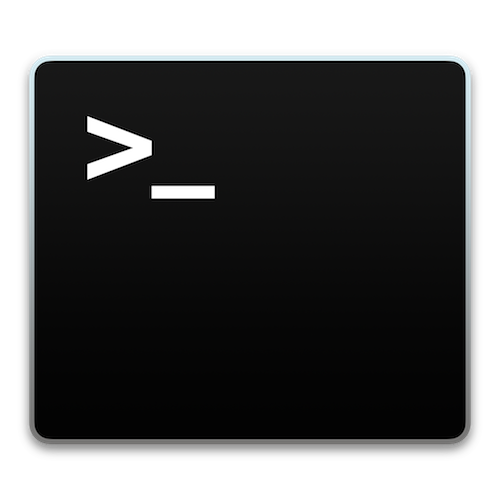
\includegraphics[scale=0.5]{terminal.png}
\end{figure}
\end{frame}
\begin{frame}{Palabras clave de Python}
Python tiene algunas palabras reservadas:\\
\begin{center}
{\tt and   \tab    del   \tab    from   \tab   not  \tab     while\\
as   \tab     elif  \tab    global  \tab  or   \tab     with\\
assert  \tab  else   \tab   if    \tab    pass  \tab    yield\\
break   \tab  except  \tab  import  \tab  print\\
class  \tab   exec   \tab   in    \tab    raise\\
continue \tab finally \tab  is    \tab    return \\
def   \tab    for   \tab    lambda  \tab  try\\
}
\end{center}
\end{frame}

\subsection{Listas}
\begin{frame}{Listas}
Una lista es una secuencia de valores ordenados
\begin{figure}
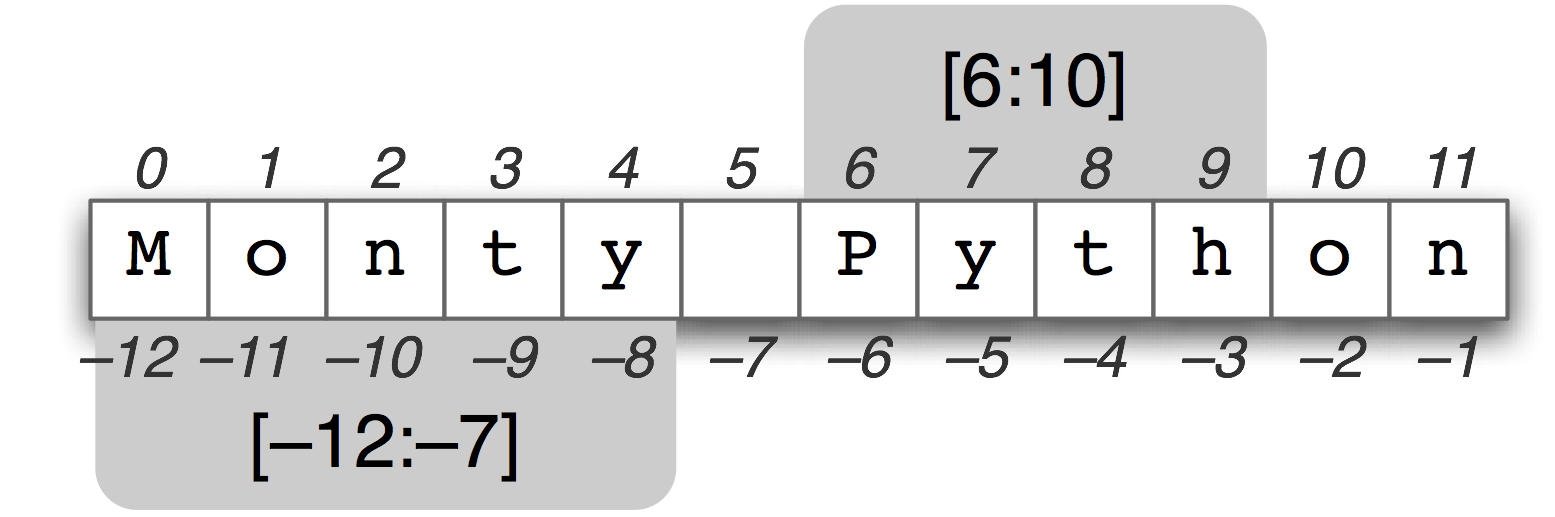
\includegraphics[scale=0.5]{lista.png}
\end{figure}
\end{frame}


\section{Funciones Integradas}

\begin{frame}{Funciones integradas (Built-in Functions)}
\begin{itemize}
\item Una {\bf función} es una secuencia de declaraciones que realizan un cálculo identificadas con un nombre.\\
\item Un {\bf módulo } es un archivo que contiene un conjunto de funciones relacionadas.
\item Algunas funciones integradas son: {\tt int(), float(), str(), type(), print, dir(), abs(), len(), open(), range()}
\end{itemize}
\end{frame}

\begin{frame}{Funciones integradas}
Volvamos  a la terminal
\begin{figure}
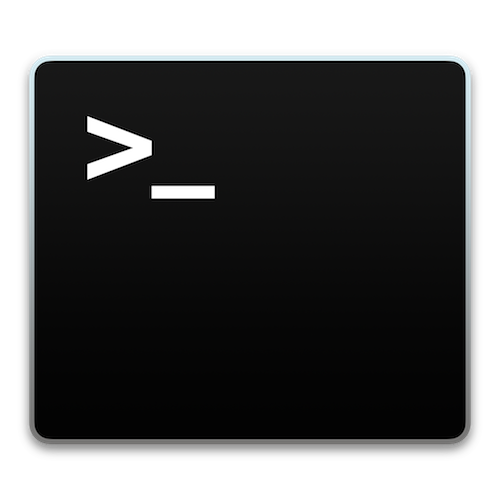
\includegraphics[scale=0.5]{terminal.png}
\end{figure}
\end{frame}

\section{Condicionales y Ciclos}
%\definecolor{bg}{rgb}{0.95,0.95,0.95}

%\defverbatim[colored]\exampleCode{

%}
\subsection{Condicionales}
\begin{frame}[fragile]{Condicionales}
La ejecución condicional permite cambiar el comportamiento de un programa dependiendo del valor de una expresión. Ej:
%\exampleCode
\begin{minted}{python}
if x > 0:
    print 'x es positivo'
elif:
    print 'x es 0 o negativo'
\end{minted}
\end{frame}

\subsection{Ciclos}
\begin{frame}[fragile]{Ciclos}
\begin{columns}
\begin{column}{0.5\linewidth}
\begin{exampleblock}{Ciclo While}
\begin{minted}{python}
n=10
while n > 0:
    print n
    n = n-1
print 'Stop!'
\end{minted}
\end{exampleblock}
\end{column}
\pause
\begin{column}{0.5\linewidth}
\begin{exampleblock}{Ciclo for}
\begin{minted}{python}
s = 'Hola Mundo!!'
for i in range(len(s)):
    print l[i]
\end{minted}
\end{exampleblock}
\end{column}
\end{columns}
\end{frame}
\end{document}